\section{Methods}
\label{sec:methods}


All experiments\footnote{\href{https://github.com/skriegman/gecco-2017}{\textbf{https://github.com/skriegman/gecco-2017}} contains the source code necessary for reproducing our results.} were performed in the open-source soft-body physics simulator  
\textit{Voxelyze}, which is described in detail in Hiller and Lipson \cite{hiller2014dynamic}.

We consider a locomotion task for soft robots composed of a $4\times4\times3$ grid of voxels (see figure \ref{fig:videos} for example). 
% nac: awkward phrasing
Each voxel within and across robots is identical with one exception:
its volume.
At any given time, a robot is completely specified by an array of \textit{resting volumes}, one for each of its 48 constituent voxels.
If the resting volumes are static across time then a robot's genotype is this array of 48 voxel volumes; however, because we enforce bilateral symmetry, a genome of half that size is sufficient.
On top of the deformation imposed by the genome, each voxel is volumetrically actuated according to a global signal that varies sinusoidally in volume over time (figure \ref{fig:illustrations}). The actuation is a linear contraction/expansion from their baseline resting volume.

Under this type of rhythmic actuation, many asymmetrical mass distributions will elicit locomotion to some extent. For instance, a simple design, with larger voxels in its front half relative to those in its back half, may be mobile when its voxels are actuated uniformly. Although this design would be rather inefficient since it most likely drags much of its body across the floor as it moves. More productive designs are not so intuitive, even with this fixed controller.

An individual is evaluated for 8 seconds, or 32 actuation cycles.
The fitness was taken to be the distance, in the positive $y$ direction, the robot's center of mass moved in 8 seconds, normalized by the robot's total volume.
Thus, a robot with volume 48 that moves a distance of 48 will have the same fitness --- a fitness of one --- as a similarly shaped but smaller robot with volume 12 that moves a distance of 12. 
Distance here is measured in units that correspond to the length of a voxel with volume one.
If, however, a robot rolls over onto its top layer of voxels it is assigned a fitness of zero and evaluation is terminated. This constraint prevents a rolling ball morphology from dominating more interesting gaits.

We have now built up all of necessary machinery of our first type of robot which we shall call the \textbf{Evo} robot.
Populations of these robots can evolve:
body plans change from generation to generation (phylogeny); but they can not develop: body plans maintain a fixed form, apart from actuation, while they behave within their lifetime (ontogeny).

We consider a second type of robot, the \textbf{Evo-Devo} robot, which inherits all of the properties of the Evo robot but has a special ability: Evo-Devo robots can develop as well as evolve.
These robots are endowed with a \textit{minimally complex} model of development in which resting volumes change linearly in ontogeny. We call this ballistic development to distinguish it from environment-mediated development.
Ballistic development is monotonic with a fixed rate predetermined by a genetic program; its onset and termination are constrained at birth and death, respectively; it is strictly linear, without mid-course correction.
The volume of the $k^{\text{th}}$ voxel in an Evo-Devo robot changes linearly from a starting volume, $v_{k0}$, to a final volume, $v_{k1}$, within the lifetime of a robot (figure \ref{fig:illustrations}). 
Accordingly, the genotype of a robot that can develop is twice as large as that of robots that cannot develop, since there are two parameters ($v_{k0}$ and $v_{k1}$) that determine the volume of the $k^{\text{th}}$ voxel at any particular time. 
Although it is important to note that the space of possible morphologies (collection of resting volumes) is equivalent both with and without development.


\begin{figure}
\centering
% \hspace{-0.3cm}
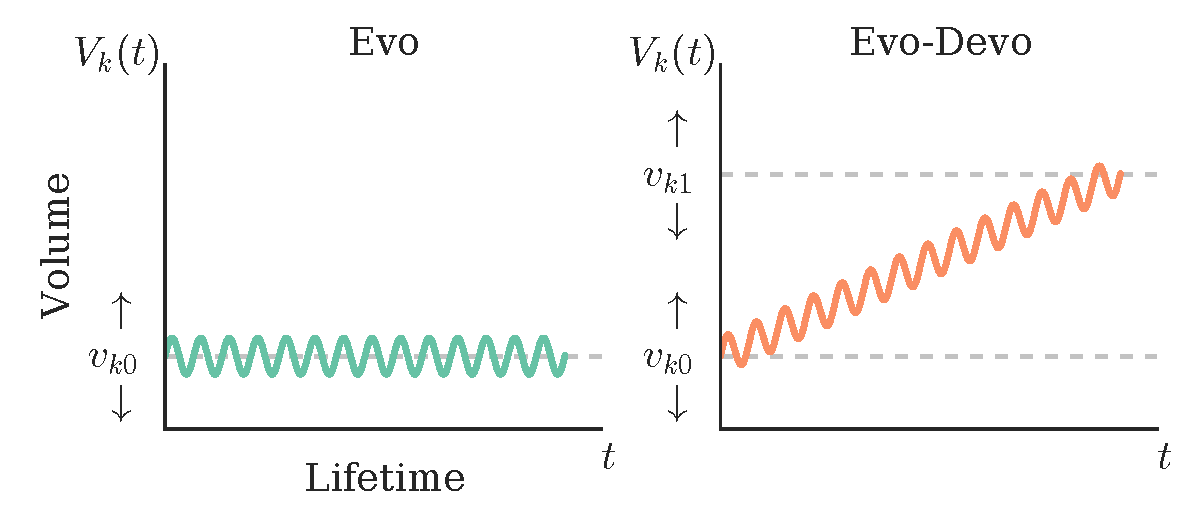
\includegraphics[width=0.75\textwidth]{Chapter03/img/high_res_illustrations_gecco}
% \vspace{-0.6cm}
\caption{\label{fig:illustrations} \textbf{The voxel picture.} The $k^{\text{th}}$ voxel in an Evo robot maintains a fixed resting volume, $v_{k0}$, throughout the robot's lifetime. Sinusoidal actuation is applied on top of the resting volume. In contrast, the $k^{\text{th}}$ voxel in an Evo-Devo robot changes linearly from a starting volume, $v_{k0}$, to a final volume, $v_{k1}$, over the robot's entire lifetime. Growth, the case when $v_{k1}>v_{k0}$, is pictured here, but shrinkage is also possible and occurs when $v_{k1}<v_{k0}$. 
When $v_{k1}=v_{k0}$, Evo-Devo voxels are behaviorally equivalent to Evo voxels. 
Voxels actuate at 4 Hz in our experiments (for 8 sec or 32 cycles) however actuation is drawn here at a lower frequency to better convey the sinusoidal volumetric structure in time.}
%nac: y-xis labels "volume", but "resting volume" is depicted.  Change label and/or add a second row with "total volume after sinusolial actuation" which shows this same picture, but with oscillating lines.  This would also help enforce the idea that while actuation and development both only affect voxel volumes, they occur on drastically different time scales.  
\end{figure}



\subsection{From gene to volume.}

%nac: awkward and confusing, just say that you use a 4x4x3, and with bilateral symmetry to result in 24 genes for Evo.  And then later say that you use 48 genes for Evo-Devo.  
% The Evo genome is a collection of 48 genes, one gene for each voxel in its $4\times4\times3$ $(x,y,z)$ body.
Like most animals, our robots are bilaterally symmetrical.
We build this constraint into our robots by constraining the 24 voxels on the positive $x$ side of the robot to be equal to their counterparts on the other side of the $y$ axis.
Instead of 48 Evo genes, therefore, we end up with 24.

A single Evo gene stores the resting length, $s_k$, of the $k^{\text{th}}$ voxel, which is cubed to obtain the \textit{resting} volume, $r_k(t)$, at any time, $t$, during the robot's lifetime.
\begin{equation} 
r_k(t)=s_k^3 \qquad k=1,2,\dots,24
\end{equation}
The resting lengths may be any real value in the range $(0.25,\; 1.75)$, inclusive. Note that the resting volume of an Evo robot does not depend on $t$, and is thus constant in ontogenetic time.

Volumetric actuation, $a(t)$ with amplitude $u$, and period $w$, takes the following general form in time.
\begin{equation}
a(t) = u* \sin(2\pi t/w)
\end{equation}
Actuation is limited to $\pm 20\%$ and cycles four times per second ($u=0.20$, $w=0.25$ sec).

However, for smaller resting volumes, the actuation amplitude is limited and approaches zero (no actuation) as the resting volume goes to its lower bound, $0.25^3$. This restriction is enforced to prevent opposite sides of a voxel from penetrating each other, effectively incurring negative volumes, which can lead to simulation instability. 
This dampening is applied only where $s_k<1$ (shrinking voxels) and accomplished through the following function.
\begin{equation}
d(s_k) = \begin{cases} 
      1 & s_k \geq 1 \\
      (4s_k-1)/3 & s_k < 1
   \end{cases}
\end{equation}
Thus $d(s_k)$ is zero when $s_k=0.25$, and is linearly increasing in $s_k\le1$. 
The true actuation, $\tilde{a}(t, s_k)$, is calculated by multiplying the unrestricted actuation, $a(t)$, by the limiting factor, $d(s_k)$.
\begin{equation}
\tilde{a}(t,s_k)=a(t)*d(s_k)
\end{equation}

Actuation is then added to the resting volume to realize the \textit{current} volume, $V_k(t)$, of the $k^{\text{th}}$ voxel of an Evo robot at time $t$.
\begin{equation} \label{eq:evo_vol}
V_k(t)=[s_k+\tilde{a}(t,s_k)]^3
\end{equation}

For Evo-Devo robots, a gene is a pair of voxel lengths $(s_{k0}, \; s_{k1})$ corresponding to the $k^{\text{th}}$ voxel's starting and final resting lengths, respectively. Thus, for a voxel in an Evo-Devo robot, the resting volume at time $t \in (0,\tau)$ is calculated as follows. 
\begin{equation} 
r_k(t)=\left[s_{k0} + \frac{t}{\tau} (s_{k1}-s_{k0})\right]^3
\end{equation}
Where the difference in starting and final scale $(s_{k1}-s_{k0})$ determines the slope of linear development which may be positive (growth) or negative (shrinkage). 
The current volume of the $k^{\text{th}}$ voxel of an Evo-Devo robot is then determined by the following.
\begin{equation}
V_k(t)=\left[ r_k^{1/3}(t) + \tilde{a}\left(t, \; r_k^{1/3}(t)\right)\right]^3
\end{equation}
Hence the starting resting volume, $v_{k0}$, and final resting volume, $v_{k1}$, are the current volumes at $t=0$ and $t=\tau$, respectively.
\begin{align}
\begin{split}
v_{k0} &= V_k(0) =  s_{k0} ^3 \\
v_{k1} &= V_k(\tau) = s_{k1} ^3
\end{split}
\end{align}
Note that an Evo gene is a special case of an Evo-Devo gene where $s_{k0}=s_{k1}$, or, equivalently, where $v_{k0}=v_{k1}$.

For convenience, let's define the current \textit{total} volume of the robot across all 48 voxels as $Q(t)$.
\begin{equation}
Q(t)=2\sum_{k=1}^{24} V_k(t)
\end{equation}
% To account for volumetric development in our objective that normalizes distance by volume, 
We track the $y$ position of the center of mass, $y(t)$, as well as the current total volume, $Q(t)$, at $n$ discrete intervals within the lifetime of a robot. Fitness, $F$, is the sum of the distance traveled in time interval, divided by the average volume in the interval.
\begin{equation} \label{eq:fitness}
F = 2 \sum_{t=1}^{n} \frac{y(t)-y(t-1)}{Q(t) + Q(t-1)}
\end{equation}
We track $y(t)$ and $Q(t)$ 100 times per second. Since robots are evaluated for eight seconds, $n=800$.

%nac: note that these values are unique for each voxel; i.e. V(t) is really V_i(t) for i=1,2,...,48

%nac: also note the explicit differnence of 24 genes for Evo and 48 genes for Evo-Devo



\subsection{A direct encoding.}


This paper differs from previous evolutionary robotics work that used Voxelyze \cite{Cheney:2013:UEE:2463372.2463404, cheney2014evolved, Cheney:2015:ESR:2739480.2754662} in that we evolve the volumes of a fixed collection of voxels, rather than the presence/absence of voxels in a bounding region. 
Another difference is that 
we do not employ the CPPN-NEAT evolutionary algorithm \cite{Stanley2007}, 
but instead use a direct encoding with bilateral symmetry about the $y$ axis.
A comparison of encodings in our scenario is beyond the scope of this paper.
However we noticed that the range of evolved morphologies here, under our particular settings, was much smaller than that of previous work which used voxels as building blocks,
and that it is easier to reach extreme volumes for individual voxels using a direct encoding. 

Apart from the difference in encoding, this work is by in large consistent with this previous work. We use the same physical environment as Cheney et al. \cite{Cheney:2013:UEE:2463372.2463404}: a wide-open flat plain. The material properties of our voxels are also consistent with the `muscle' voxel type from the palette in this work;  
although these voxels had a fixed resting volume of one ($s_k=1$ for all $k$).
% Our developmental mechanism is strongly based on Corucci et al. \cite{corucci2016material}, which used volumetric deformation in a closed-loop pointing task.

%nac: this environment is a standard one and was not introduced by Cheney et al. (though we were the first to evolve soft 



\subsection{Evolutionary search.}


We employ a standard evolutionary algorithm, Age-Fitness-Pareto Optimization (AFPO, \cite{Schmidt2011}), which uses the concept of Pareto dominance and an objective of age (in addition to fitness) intended to promote diversity among candidate designs. For 30 runs, a population of 30 robots is evolved for 2000 generations.
Every generation, the population is first doubled by creating modified copies of each individual in the population. Next, an additional random individual is injected into the population. Finally, selection reduces the population down to its original size according to the two objectives of fitness (maximized) and age (minimized).

% Whereas Evo robots have a single parameter per voxel dictating a static volume, Evo-Devo robots have two parameters per voxel dictating their starting and final volumes.
% Despite this imbalance, the same number of parent voxels are mutated, on average, in both Evo and Evo-Devo children.
% Mutations to a particular voxel parameter follow a normal distribution ($\sigma=0.75$) and are considered hierarchically, first at the volume parameter level and then at the voxel level.
% This process is straight forward for Evo children: simply visit each voxel (on the positive $x$ side) of the parent and, with probability 0.5, mutate its single parameter value.
% An addition step is required to create an Evo-Devo child.
% First, by flipping two separate metaphorical (but fair) coins, select whether mutations will effect just the initial volumes (Heads, Tails), just the final volumes (Tails, Heads), or both (Heads, Heads). If both coins turn up Tails, then a third and final coin determines the selection of just initial volumes (Heads) or just final volumes (Tails).
% Then, for each parameter whose mutational coin turned up Heads and was thus selected for mutation, apply the same mutation process as before in Evo robots: loop through each voxel of the parent and, with probability 0.5, mutate the selected parameter. 
% Therefore, \textit{for each parameter}, the expected number of voxels mutated in Evo and Evo-Devo robots is equivalent. 

%nac:  explain simpler as something like: (1) choosing what parameter types to mutate, and (2) choosing which voxels to mutate.  Flip a coin for each parameter to be mutated (if neither will be mutated, flip a final coin to choose one or the other).  This results in a 25% chance of mutating both, and a 37.5% chance of mutating each of the two individual parameters alone.

The same number of parent voxels are mutated, on average, in both Evo and Evo-Devo children.
Mutations follow a normal distribution ($\sigma=0.75$) and are applied by first choosing what parameter types to mutate, and then choosing which voxels to mutate.
For Evo robots, we simply visit each voxel (on the positive $x$ side) of the parent and, with probability 0.5, mutate its single parameter value.
For Evo-Devo parents, we flip a coin for each parameter to be mutated (if neither will be mutated, flip a final coin to choose one or the other).  
This results in a 25\% chance of mutating both, and a 37.5\% chance of mutating each of the two individual parameters alone.
Then we apply the same mutation process as before in Evo robots: loop through each voxel of the parent and, with probability 0.5, mutate the selected parameter(s).


% This mutation procedure is designed to be fair across our treatments while facilitating a test of our hypothesis that late-in-life mutations (to final volumes) have smaller phenotypic impact than early-in-life mutations (to initial volumes). We could have applied mutations in reverse hierarchy--- considering voxel location first and then its volume parameters. This would enforce equivalence in the average number of voxels mutated \textit{overall} between treatments, but would, to a much greater extent, mix early-in-life and late-in-life mutations within a single individual which could make testing our hypothesis more difficult using individual-level statistics like fitness.

% % nac: the above wording makes it sound as though this is our main hypothesis, which I do not believe it is... 

\subsection{An artificially rugged landscape.}

We did not fine-tune the mutation hyperparameters (scale and probability), but intentionally chose a relatively high probability of mutation in order to elicit a large mutational impact in an attempt to render evolutionary search more difficult. 
This removes easy to follow gradients in the search space --- `compressing' gentle slopes into abrupt cliffs --- which make `good designs' more difficult to find.  Any one of these good solutions then, to a certain extent, become like Hinton \& Nowlan's `needle in a haystack' \cite{hinton1987learning}.

Note that there are other ways to enforce rugged fitness landscapes, and such landscapes are naturally occurring in many systems, though our particular task/environment is not one of them. Future work should investigate these tasks and environments with a fine-tuned mutation rate. 

% nac: note that there are other way to enforce rugged landscapes, and that such landscapes are naturally occuring in many systems without the need to intentially create it (though this is not one of them) -- and that future work should investigate these tasks and environments with a fine-tuned mutation rate. 
